% TeXLocal test document: a long article.
% What to try with it:
%  - The File Outline: every heading level, a starred section, one with a
%    short title, an empty \subsection{} ("Untitled Subsection"), and a
%    commented-out \section that must not appear.
%  - The breadcrumb above the source, moving the caret between sections.
%  - SyncTeX both ways: Command-click in the PDF, and the source's jump to PDF.
%  - Find in the source and in the PDF: section "Search Targets" has "needle"
%    in several cases and forms (for Match Case and Whole Words).
%  - Scrolling, zoom and fit on about 20 pages; links (hyperref's boxes).
%  - Word count and line count in the status bar.
\documentclass[11pt]{article}
\usepackage[T1]{fontenc}
\usepackage{amsmath,amssymb,amsthm}
\usepackage{graphicx}
\usepackage{booktabs}
\usepackage{tikz}
\usepackage{lipsum}
\usepackage{hyperref}

\newtheorem{theorem}{Theorem}[section]
\newtheorem{lemma}[theorem]{Lemma}
\theoremstyle{definition}
\newtheorem{definition}[theorem]{Definition}

\title{A Test Article for TeXLocal}
\author{The TeXLocal Test Documents}
\date{\today}

\begin{document}

\maketitle

\begin{abstract}
This article exists to be edited, compiled and broken. It has every heading. \bibliography{}
level the outline shows, some mathematics, a table, two figures, nested lists
and enough filler text to scroll through. Nothing in it is meant to be read.
\end{abstract}

\tableofcontents

\section{Introduction}\label{sec:intro}
This is the introduction. Section~\ref{sec:maths} has the mathematics,
Table~\ref{tab:results} a table and Figure~\ref{fig:tikz} a drawing. The
project's website would be at \url{https://example.com}, and a footnote
follows.\footnote{A footnote, for SyncTeX to find at the foot of the page.}

\subsection{Motivation}
\lipsum[1]

\subsubsection{A Deeper Heading}
\lipsum[2]

\paragraph{A Paragraph Heading}
The deepest level the outline shows. \lipsum[3][1-4]

\section*{A Starred Section}
Starred headings still appear in the outline, unnumbered.
\lipsum[4]

\section[Short Title]{A Section Whose Full Title Is Much Too Long to Fit in the Breadcrumb Bar Above the Source}
The outline and the breadcrumb show the full title; the table of contents shows
the short one.

\subsection{}
% An empty title: the outline names it by its kind, "Untitled Subsection".
This subsection has no title.

% \section{Commented Out}
% This heading is commented out, so it must not appear in the outline.

\section{Mathematics}\label{sec:maths}

\begin{definition}
A \emph{test document} is one whose content is beside the point.
\end{definition}

\begin{theorem}[Pythagoras]\label{thm:pythagoras}
For a right triangle with legs $a$ and $b$ and hypotenuse $c$,
\begin{equation}\label{eq:pythagoras}
  a^2 + b^2 = c^2.
\end{equation}
\end{theorem}

\begin{proof}
By Equation~\eqref{eq:pythagoras}, which is circular, but this is a test.
\end{proof}

\begin{lemma}
The Gaussian integral is
\[
  \int_{-\infty}^{\infty} e^{-x^2}\,dx = \sqrt{\pi}.
\]
\end{lemma}

Aligned equations:
\begin{align}
  f(x) &= \sum_{n=0}^{\infty} \frac{f^{(n)}(0)}{n!}\, x^n \label{eq:taylor}\\
  e^{i\pi} + 1 &= 0 \\
  \nabla \times \mathbf{B} &= \mu_0 \mathbf{J} + \mu_0 \varepsilon_0 \frac{\partial \mathbf{E}}{\partial t}
\end{align}

A matrix, $\det A = ad - bc$ for
$A = \begin{pmatrix} a & b \\ c & d \end{pmatrix}$, and a cases block:
\[
  |x| = \begin{cases} x & x \ge 0, \\ -x & x < 0. \end{cases}
\]

\section{Tables and Figures}

\begin{table}[ht]
  \centering
  \caption{Some results, in a booktabs table.}\label{tab:results}
  \begin{tabular}{lrrr}
    \toprule
    Method & Precision & Recall & $F_1$ \\
    \midrule
    Baseline & 0.71 & 0.64 & 0.67 \\
    Ours     & 0.83 & 0.79 & 0.81 \\
    Oracle   & 1.00 & 1.00 & 1.00 \\
    \bottomrule
  \end{tabular}
\end{table}

\begin{figure}[ht]
  \centering
  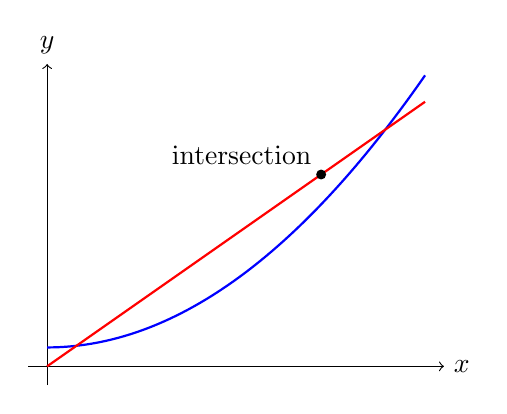
\begin{tikzpicture}[scale=1.2]
    \draw[->] (-0.2,0) -- (4.2,0) node[right] {$x$};
    \draw[->] (0,-0.2) -- (0,3.2) node[above] {$y$};
    \draw[thick, blue, domain=0:4, samples=60] plot (\x, {0.18*\x*\x + 0.2});
    \draw[thick, red, domain=0:4] plot (\x, {0.7*\x});
    \fill (2.9,2.03) circle (1.5pt) node[above left] {intersection};
  \end{tikzpicture}
  \caption{A TikZ drawing.}\label{fig:tikz}
\end{figure}

\begin{figure}[ht]
  \centering
  \includegraphics[width=0.5\linewidth]{example-image-a}
  \caption{An image from TeX Live's \texttt{mwe} package.}\label{fig:image}
\end{figure}

\section{Lists}
\begin{itemize}
  \item A bullet.
  \item A bullet with a nested list:
  \begin{enumerate}
    \item first,
    \item second,
    \begin{description}
      \item[Term] its description.
    \end{description}
  \end{enumerate}
  \item A last bullet.
\end{itemize}

\section{Long Text for Scrolling}
\subsection{Filler One}   \lipsum[5-12]
\subsection{Filler Two}   \lipsum[13-20]
\subsection{Filler Three} \lipsum[21-28]
\subsection{Filler Four}  \lipsum[29-36]
\subsubsection{Filler Four, Deeper} \lipsum[37-44]
\subsection{Filler Five}  \lipsum[45-52]
\subsection{Filler Six}   \lipsum[53-60]

\section{Search Targets}\label{sec:search}
The word needle appears here, then Needle with a capital, NEEDLE in capitals,
needles in the plural and haystackneedle inside another word. A needle, a
needle and one more needle. Match Case finds only the lower-case ones; Whole
Words skips the plural and the one inside another word.

\appendix
\section{An Appendix}
\lipsum[61-64]

\end{document}
